% -*- mode: LaTeX; coding: utf-8 -*-
% Typeset with: XeLaTeX

\documentclass{beamer}
\mode<presentation>
{
  \usetheme[progressbar=foot,numbering=fraction,background=light]{metropolis} 
  \usecolortheme{default} % or try albatross, beaver, crane, ...
  \usefonttheme{default}  % or try serif, structurebold, ...
  \setbeamertemplate{navigation symbols}{}
  \setbeamertemplate{caption}[numbered]
  %\setbeamertemplate{frame footer}{My custom footer}
}
\centering

\usepackage{graphicx}
\graphicspath{ {./fp_figures/} }
\usepackage{hyperref,xcolor}
\newcommand{\link}[2]{\href{#1}{\textcolor{blue}{\underline{#2}}}}

% Main document
\begin{document}
\title{DeepSite: NNets for binding site prediction}
\subtitle{Algorithms in Structural Bioinformatics}
\author{Thomas Pappas}
%\date{4 March 2020}
\maketitle

\begin{frame}{Agenda}
  \tableofcontents[hideallsubsections]
\end{frame}

\section{What is the project about?}

\begin{frame}{What is DeepSite?}
  \begin{block}{DeepSite}
    Protein-binding site \emph{predictor} using 3D-convolutional neural networks
    \begin{itemize}
      \item Using DCNN due to an existing database of 7622 proteins from scPDB to train the NNet
      \item Superior performance to two other competitive algorithmic strategies
      \item Available online at \link{https://www.playmolecule.com/deepsite/}{https://www.playmolecule.com/deepsite/}
    \end{itemize}
  \end{block}
\end{frame}

\begin{frame}{Aim and objectives}
  \begin{block}{Review}
    How does DeepSite takes a PDB structure and implements a DCNN on it to predict binding sites?
  \end{block}
  \begin{block}{Confirm}
    Test the algorithm with more recent available data.
  \end{block}
  \begin{block}{Compare}
    See the algorithm's performance compared to other binding site prediction ones, i.e. fpocket
  \end{block}
\end{frame}

\section{The DeepSite algorithm}

\begin{frame}{DeepSite Algorithm summary}
  \begin{block}{Algorithm summary}
    \begin{itemize}
      \item Takes as input a protein ID or a PDB file
      \item Translates the molecular structures to 8 grids representing molecular properties
      \begin{itemize}
        \item The 8 grids are basically channels that NNs take as input
      \end{itemize}
      \item Takes $16 \times 16 \times 16$ \AA$^3$ subgrids from the 8 channels as input for the Deep Convolutional Neural Network (DCNN)
      \item Returns a list of predicted points to be binding sites, along with their success score
    \end{itemize}
  \end{block}
\end{frame}

\begin{frame}{Example of a 6FAT protein}
  \begin{figure}[h]
    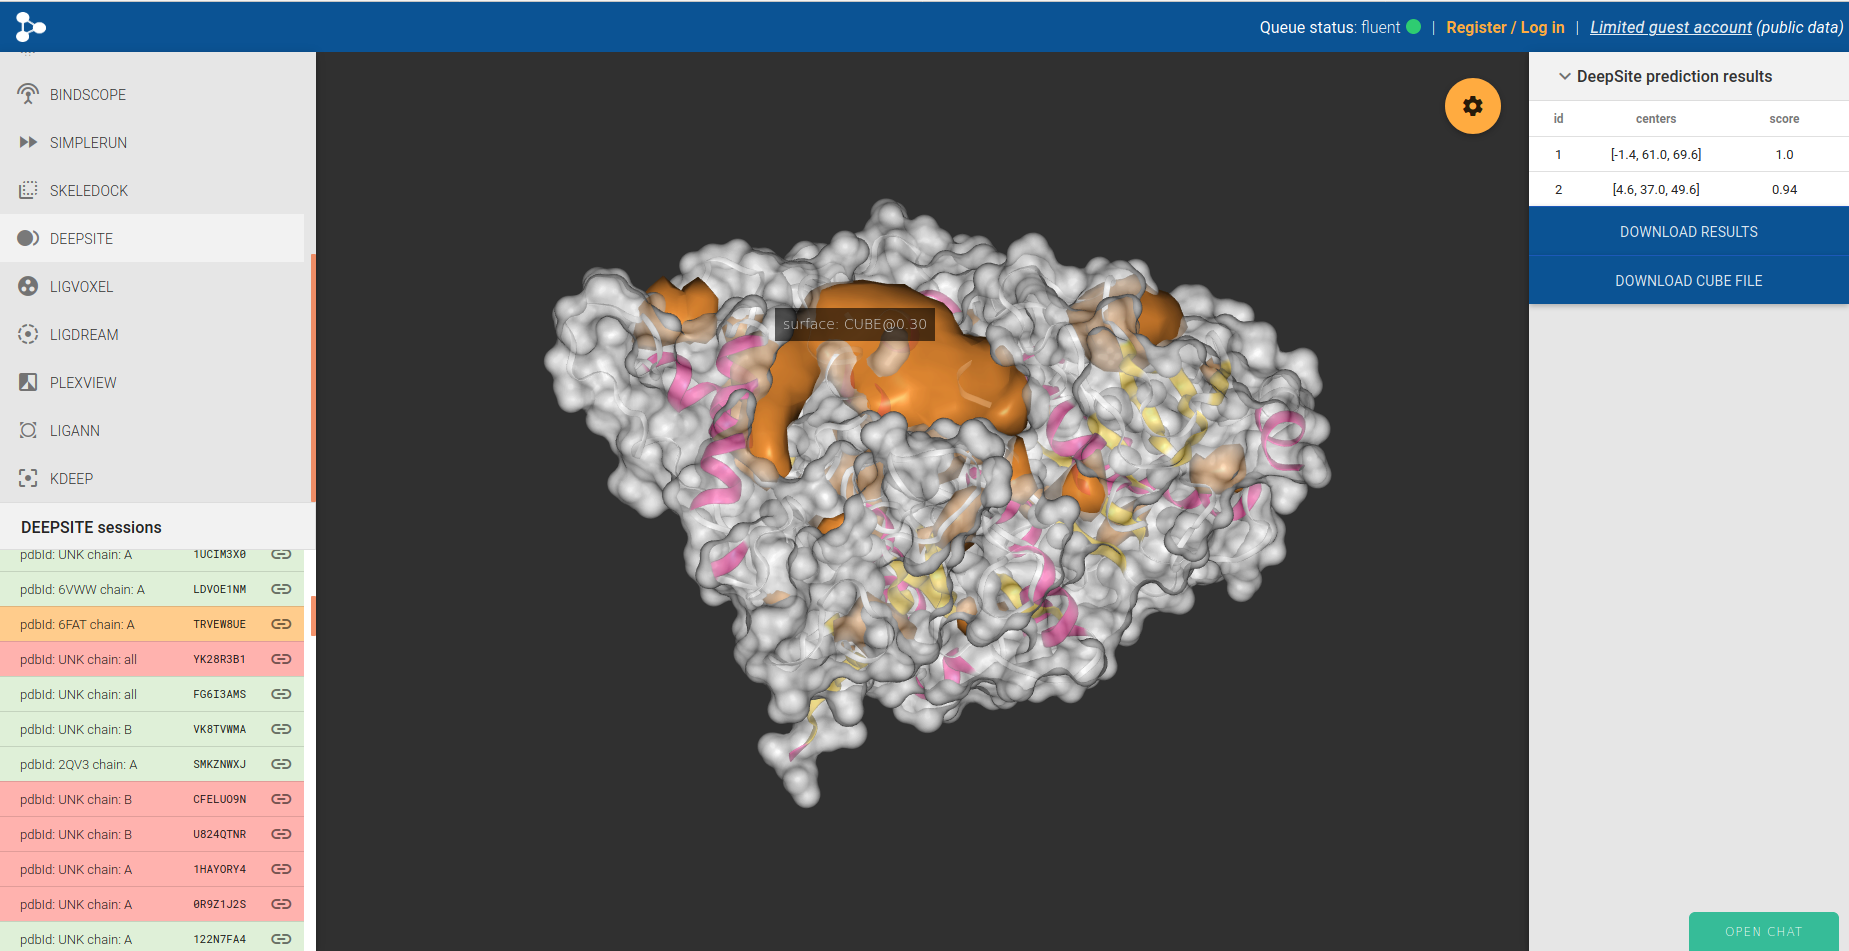
\includegraphics[width=1\textwidth]{deepsite_6fat_result}
    \caption{The 6FAT protein submitted in the \link{https://www.playmolecule.com/deepsite/}{DeepSite web app}}
  \end{figure}
\end{frame}

\subsection{Translating PDB to NNet channels}

\begin{frame}{Translating PDB to NN channels}
  \begin{block}{Parsing the PDB data}
    \begin{itemize}
      \item Parse the atom coordinates from the PDB data
      \begin{itemize}
        \item Use of the HTMDs (Doerr et al., 2016) Python package
      \end{itemize}
      \item Use the AutoDock 4 tables (Tables \ref{table:1} \& \ref{table:2}) and create 8 \emph{filtered set of atoms}, one for each protein property
      \item Consider the space grid containing the protein
      \begin{itemize}
        \item Grid is split to $1 \times 1 \times 1 $ \AA$^3$ voxels
        \item $+8$\AA \;for the cases where the binding pockets are on the edge
      \end{itemize}
    \end{itemize}
  \end{block}
\end{frame}

\begin{frame}{AutoDock 4 tables}
  \begin{columns}
    \begin{column}{.4\textwidth}
      \begin{tiny}
      \begin{table}
      \caption{Atom types}
      \label{table:1}
      \begin{tabular}{ l l }
        \hline
        Element & Description \\
        \hline
        C & Non H-bonding aliphatic carbon \\
        A & Non H-bonding aromatic carbon \\
        NA & Acceptor 1 H-bond nitrogen \\
        NS & Acceptor S Spherical nitrogen \\
        OA & Acceptor 2 H-bonds oxygen \\
        OS & Acceptor S Spherical oxygen \\
        SA & Acceptor 2 H-bonds sulfur \\
        HD & Donor 1 H-bond hydrogen \\
        HS & Donor S Spherical hydrogen \\
        MG & Non H-bonding magnesium \\
        ZN & Non H-bonding zinc \\
        MN & Non H-bonding manganese \\
        CA & Non H-bonding calcium \\
        FE & Non H-bonding iron \\
        \hline
      \end{tabular}
      \end{table}
      \end{tiny}
    \end{column}
    \begin{column}{.6\textwidth}
      \begin{tiny}
      \begin{table}
      \caption{Property-atom type correspondence}
      \label{table:2}
      \begin{tabular}{ l l }
        \hline
        Property & Rule \\
        \hline
        Hydrophobic & atom type C or A \\
        Aromatic & atom type A \\
        Hydrogen bond acceptor & atom type NA or NS or OA or OS or SA \\
        Hydrogen bond donor & atom type HD or HS with O or N partner \\
        Positive ionizable & atom with positive charge \\
        Negative ionizable & atom with negative charge \\
        Metal & atom type MG or ZN or MN or CA or FE \\
        Excluded volume & all atom types \\
      \end{tabular}
      \end{table}
      \end{tiny}
    \end{column}
  \end{columns}
  Table 1, Table 2, 10.1093/bioinformatics/btx350
\end{frame}

\begin{frame}{Translating PDB to NN channels}
  \begin{block}{Atom occupancy}
    We calculate the probability of an atom to exist near the center of a voxel by using the pair correlation function
    \[
      g(r) = exp(-\beta V(r))
    \]
    where $V(r) = \epsilon (r_{vdw}/r)^{12}$ and by taking $\epsilon = \beta^{-1}$ we get the \emph{single atom occupancy estimate} to be
    \[
      n(r) = 1 - exp(-(r_{vdw}/r)^{12})
    \]
  \end{block}
  \begin{block}{Building the NN channels}
    Create a channel (3D matrix) for each of the 8 atom sets, and for each voxel assign the probability of the voxel having an atom of that property (Figure 2)
  \end{block}
\end{frame}

\begin{frame}{Translating PDB to NN channels}
  \begin{figure}[h]
    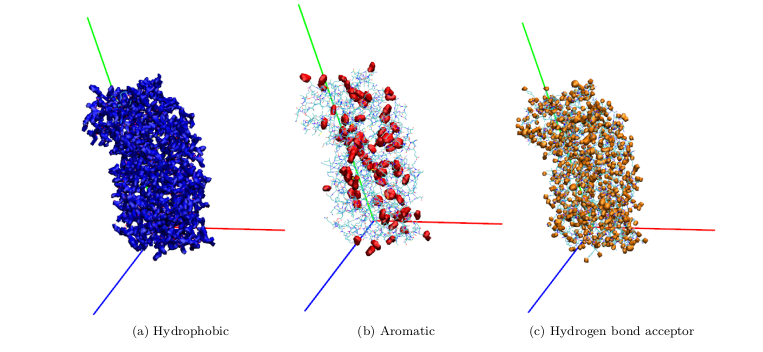
\includegraphics[width=1\textwidth]{deepsite_protein_property_channels}
    \caption{Visual representations of descriptor channels (3/8) for PDB ID 4NIE, Figure S2, 10.1093/bioinformatics/btx350}
  \end{figure}
\end{frame}

\subsection{NNet design}

\begin{frame}{NNet design}
  \begin{figure}[h]
    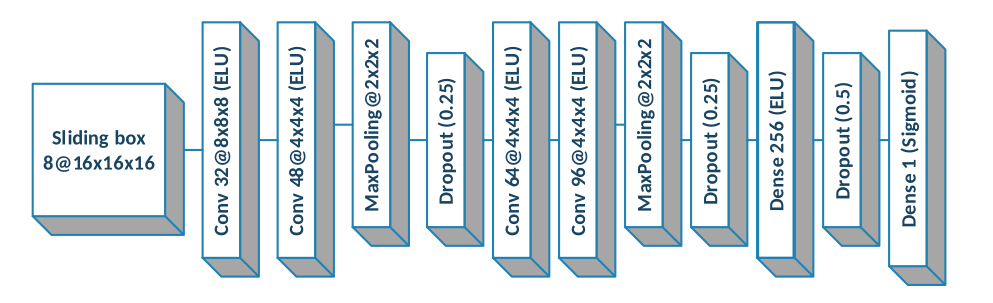
\includegraphics[width=1\textwidth]{deepsite_dcnn_architecture}
    \caption{DeepSite’s internal DCNN architecture, Fig. 2, 10.1093/bioinformatics/btx350}
  \end{figure}
\end{frame}

\begin{frame}{NNet training}
  \begin{block}{Training}
    \begin{itemize}
      \item Input subgrids of $16 \times 16 \times 16$ \AA$^3$
      \item Step of 4 voxels
    \end{itemize}
  \end{block}
  \begin{block}{Success criteria for a subgrid}
    Geometric center is closer than 4 Å to the pocket geometric center
  \end{block}
\end{frame}

\begin{frame}{NNet properties}
  \begin{block}{Layers}
    \begin{itemize}
      \item 4 Convolutional Layers
      \item Max Pooling and Dropout layers after each 2
      \item Sigmoid activation function at the end to get a probability value
    \end{itemize}
  \end{block}
  \begin{block}{But why?}
    \begin{itemize}
      \item Common practices in the ML community
      \item Simplified model due to scarcity of data
    \end{itemize}
  \end{block}
  \begin{block}{Issues?}
    \begin{itemize}
      \item Class imbalance problem (many 0 cases)
      \begin{itemize}
        \item Undersampling of dataset
      \end{itemize}
    \end{itemize}
  \end{block}
\end{frame}

\begin{frame}{NNet end result}
  The algorithm will run for all subgrids and will output a full probability map for all voxels.
  So for a protein
  \begin{itemize}
    \item returns a volumetric map of predicted binding sites
    \item uses the Mean-Shift clustering algorithm to distinguish different binding sites in that protein
  \end{itemize}
\end{frame}

\subsection{Evaluating the NNet model}

\begin{frame}{10-fold cross-validation}
  Dataset of 7622 scPDB structures
  \begin{block}{Steps}
    \begin{itemize}
      \item Split the training dataset to 10 (equal size) sets
      \item Consider one as a testing set and the rest as training ones and evaluate its success
      \item Cycle through each set and repeat the evaluation
      \item Final result is the average of all above evaluations
    \end{itemize}
  \end{block}
  \begin{block}{Why $k$-fold cross validation?}
    \begin{itemize}
      \item Common practice for validating NNet models
      \item Limits the possibility of over-fitting
    \end{itemize}
  \end{block}
\end{frame}

\begin{frame}{Evaluation metrics}
  \begin{block}{Distance to the center of the binding site (DCC)}
    A prediction is successful is closer than a given threshold to the real binding site
    \begin{itemize}
      \item Values uses range from 4 to 20 \AA
      \item Ignores the shape of the predicted pocket
    \end{itemize}
  \end{block}
  \begin{block}{Discretized volumetric overlap (DVO)}
    Discretize protein space to $1 \times 1 \times 1$ \AA$^3$ voxels and calculate the Jaccard index
    \[
      J = \frac{\#|V_r \cap V_p|}{\#|V_r \cup V_p|}
    \]
    $V_r$: set of voxels in real binding pocket\\
    $V_p$: set of voxels in predicted binding pocket
    \begin{itemize}
      \item Takes into account the shape of the predicted pocket
    \end{itemize}
  \end{block}
\end{frame}

\section{Confirming for old and new data}

\begin{frame}{Method}
  \begin{block}{sc-PDB}
    When DeepSite was published, sc-PDB contained 9283 entries;\\
    as of today it has 16034
  \end{block}
  \begin{block}{Steps for evaluating results (for a protein)}
    \begin{itemize}
      \item Download the sc-PDB entries
      \begin{itemize}
        \item (Real) Binding site atom info contained in "site.mol2" file
      \end{itemize}
      \item Run the DeepSite algorithm from the \link{https://www.playmolecule.com/deepsite/}{online web app} using the PDB ID and the chain from the sc-PDB info
      \item Calculate the geometric center of the real binding site and its distance from the DeepSite output
      \begin{itemize}
        \item In case of multiple ouputs, keep the one with min distance
        \item Distance should be $<20$\AA
      \end{itemize}
    \end{itemize}
    Test the method with proteins from the training set, and then evaluate with the newer additions
  \end{block}
\end{frame}

\begin{frame}{Testing for proteins from the training set}
  \begin{tiny}
  \begin{table}
  \caption{Success evaluation for proteins in the training set}
  \label{table:3}
  \begin{tabular}{ c | c | c | c | c }
    PDB ID (chain) & scPDB ID & DeepSite site prediction & DeepSite score & distance to real (\AA) \\
    \hline
    2GQ3 (A) & 2gq3\_1 & $(39.08, 40.04, 83.57)$ & $0.999$ & $18.86$ \\
    1HT2 (H) & 1ht2\_4 & $(100.75, 84.69, 105.11)$ & $0.999$ & $2.98$ \\
    3AHN (A) & 3ahn\_1 & $(18.3, -0.36, 4.47)$ & $0.999$ & $4.02$ \\
    1RBQ (B) & 1rbq\_2 & $(-42.67, 44.16, 11.63)$ & $0.997$ & $4.02$ \\
    %1NLY (A) & 1nly\_1
    %1OO6 () & 1oo6_1
    1RJ9 (A) & 1rj9\_1 & $(30.88, 8.67, 27.27)$ & $0.995$ & $2.83$ \\
  \end{tabular}
  \end{table}
  \end{tiny}
\end{frame}

\begin{frame}{Testing for newer additions to the sc-PDB}
  \begin{tiny}
  \begin{table}
  \caption{Success evaluation for newer proteins}
  \label{table:4}
  \begin{tabular}{ c | c | c | c | c }
    PDB ID (chain) & scPDB ID & DeepSite site prediction & DeepSite score & distance to real (\AA) \\
    \hline
    10MH (A) & 10mh\_1 & $(-23.23, 45.71, 89.51)$ & $0.99$ & $17.91$ \\
    2QJP (G) & 2qjp\_6 & $(73.90, 28.70, 35.20)$ & $0.99$ & $3.87$ \\
    2QJP (J) & 2qjp\_7 & $(75.51, -12.29, 33.10)$ & $0.99$ & $5.27$ \\
    4YLH (K) & 4ylh\_11 & $(64.01, 100.21, -24.34)$ & $0.999$ & $4.016$
  \end{tabular}
  \end{table}
  \end{tiny}
\end{frame}

\section{Comparing with fpocket}

\begin{frame}{Method}
  \begin{block}{fpocket}
    fpocket is a very fast open source protein pocket detection algorithm based on Voronoi tessellation
    \begin{itemize}
      \item \link{https://github.com/Discngine/fpocket}{fpocket GitHub repo}
    \end{itemize}
  \end{block}
  \begin{block}{Steps for evaluating results (for a protein)}
    \begin{itemize}
      \item Download the PDB file
      \item Run the fpocket command for the above PDB file
      \begin{itemize}
        \item Default script options
      \end{itemize}
      \item Take the 1st pocket result (highest score)
      \item Calculate geometric center and distance from real binding site as before
    \end{itemize}
  \end{block}
\end{frame}

\begin{frame}{Comparing prediction results}
  \begin{tiny}
  \begin{table}
  \caption{Comparison of DeepSite and fpocket algorithms}
  \label{table:5}
  \begin{tabular}{ c | c | c | c | c }
    PDB ID & sc-PDB ID & fpocket pocket & fpocket score & distance to real (\AA) \\
    \hline
    2GQ3 & 2gq3\_1 & $(49.60, 27.14, 84.73)$ & $0.99$ & $4.22$ \\
    1RJ9 & 1rj9\_1 & $(32.63, 5.71, 33.32)$ & $0.99$ & $4.62$ \\
    10MH & 10mh\_1 & $(-15.86, 31.04, 91.05)$ & $0.263$ & $6.78$ \\
    2QJP & 2qjp\_7 & $(71.70, -16.21, 32.28)$ & $0.984$ & $1.15$
  \end{tabular}
  \end{table}
  \end{tiny}
\end{frame}

\section{Comments}

\begin{frame}{Comments}
  Overall: \textbf{It works!}
  
  \begin{block}{However}
    \begin{itemize}
      \item Not all results can be verified
      \begin{itemize}
        \item e.g. protein 2QJP has $10+$ predicted pockets but only $2$ can be verified by sc-PDB
      \end{itemize}
    \end{itemize}
  \end{block}
  
  \begin{block}{Comparison to fpocket}
    \begin{itemize}
      \item The DeepSite algorithm seems to indeed score much better in most proteins
      \item Regarding the distance from the real binding site, however, fpocket seems to perform better
    \end{itemize}
  \end{block}
\end{frame}

\begin{frame}{Contact details}
  \begin{center}
    Thomas Pappas\\
    \link{mailto:thpappas@di.uoa.gr}{thpappas@di.uoa.gr}
  \end{center}
\end{frame}

\end{document}
